\documentclass[border=10pt]{standalone}
\usepackage[T1]{fontenc}
\usepackage{helvet}
\renewcommand{\familydefault}{\sfdefault}
\usepackage{tikz}
\usetikzlibrary{arrows.meta, positioning, shapes.geometric, fit, calc}

\definecolor{modelblue}{HTML}{4A90D9}
\definecolor{modelfill}{HTML}{DBEAFE}
\definecolor{choiceorange}{HTML}{E8913A}
\definecolor{choicefill}{HTML}{FEF3C7}
\definecolor{utilgreen}{HTML}{34A853}
\definecolor{utilfill}{HTML}{D1FAE5}
\definecolor{arrowgray}{HTML}{6B7280}
\definecolor{textgray}{HTML}{374151}

\begin{document}
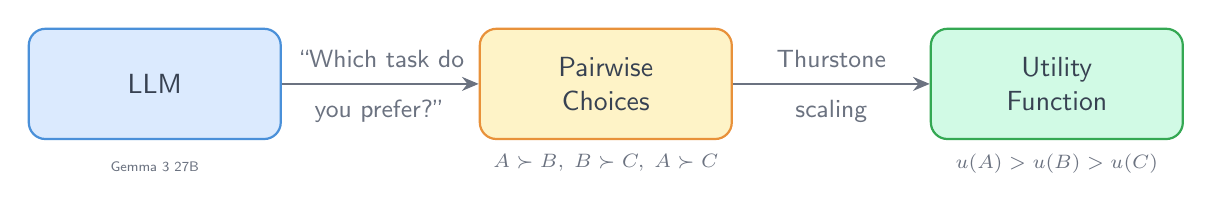
\begin{tikzpicture}[
    node distance=2.5cm,
    every node/.style={font=\sffamily, text=textgray},
    box/.style 2 args={
        draw=#1, fill=#2,
        rounded corners=6pt,
        minimum width=3.2cm, minimum height=1.4cm,
        line width=0.8pt,
        align=center,
        font=\sffamily\normalsize
    },
    arr/.style={
        -{Stealth[length=6pt, width=5pt]},
        line width=1pt,
        color=arrowgray
    },
    label/.style={
        font=\sffamily\small,
        text=arrowgray,
        align=center
    }
]

% Nodes
\node[box={modelblue}{modelfill}] (model) {LLM};

\node[box={choiceorange}{choicefill}, right=of model] (choices) {Pairwise\\Choices};

\node[box={utilgreen}{utilfill}, right=of choices] (utility) {Utility\\Function};

% Arrows
\draw[arr] (model) -- (choices)
    node[label, midway, above, yshift=2pt] {``Which task do}
    node[label, midway, below, yshift=-2pt] {you prefer?''};

\draw[arr] (choices) -- (utility)
    node[label, midway, above, yshift=2pt] {Thurstone}
    node[label, midway, below, yshift=-2pt] {scaling};

% Small illustration inside model box
\node[below=0.15cm of model.south, font=\tiny\sffamily, text=arrowgray] {Gemma 3 27B};

% Small illustration inside choices: A > B
\node[below=0.05cm of choices.south, font=\scriptsize\sffamily, text=arrowgray]
    {$A \succ B,\; B \succ C,\; A \succ C$};

% Small illustration inside utility: u(·)
\node[below=0.05cm of utility.south, font=\scriptsize\sffamily, text=arrowgray]
    {$u(A) > u(B) > u(C)$};

\end{tikzpicture}
\end{document}
